\documentclass[12pt,a4paper,oneside]{report}
\usepackage[utf8]{inputenc}
\usepackage[english]{babel}
\usepackage{t1enc}
\usepackage{amsmath}
\usepackage{amssymb}
\usepackage{enumerate}
\usepackage{graphicx}
\usepackage{epsfig}
\usepackage{listings}
\usepackage{color}
\usepackage[usenames,dvipsnames]{xcolor}
\usepackage{lastpage}
\usepackage{anysize}
\usepackage{sectsty}
\usepackage{setspace}
\usepackage[hang]{caption}
\usepackage{hyperref}
\usepackage{verbatim}
\usepackage{array,booktabs}
\usepackage{colortbl}
\usepackage{xcolor}
\usepackage{ctable}
\usepackage{minted}
\usepackage{fancyvrb}

\VerbatimFootnotes

\definecolor{bg}{rgb}{0.86,0.86,0.86}
\usemintedstyle{borland}

\newcommand{\docAuthor}{Sándor Balázs}
\newcommand{\docTitle}{Sentiment Analysis Using LingPipe}
\newcommand{\resources}{../resources}

\pagestyle{plain}
\setlength{\parindent}{12pt}
\setlength{\parskip}{0pt}

\marginsize{25mm}{25mm}{15mm}{15mm}
\setcounter{secnumdepth}{0}
\sectionfont{\large\upshape\bfseries}
\setcounter{secnumdepth}{3}
\singlespacing
\frenchspacing

\hypersetup{
  bookmarksopen=true,
  unicode=false,
  pdfencoding=auto,
  pdftitle={\docTitle},
  pdfauthor={\docAuthor},
  pdfnewwindow=true,
  colorlinks=true,
  linkcolor=Black,
  citecolor=Black,
  filecolor=Black,
  urlcolor=Blue,
}

\lstset{
  basicstyle=\scriptsize\ttfamily,
  keywordstyle=\color{black}\bfseries\underbar,
  identifierstyle=,
  commentstyle=\color{white},
  stringstyle=\scriptsize\sffamily,
  showstringspaces=false,
  aboveskip=3pt,
  belowskip=3pt,
  columns=fixed,
  backgroundcolor=\color{lightgray},
}

\newcommand{\code}[1]{{\upshape\ttfamily\scriptsize\indent #1}}
\newcommand{\figref}[1]{\ref{fig:#1}.}
\renewcommand{\eqref}[1]{(\ref{eq:#1})}
\newcommand{\listref}[1]{\ref{listing:#1}.}
\newcommand{\sectref}[1]{\ref{sect:#1}}
\newcommand{\tabref}[1]{\ref{tab:#1}.}
\newcommand{\lstref}[1]{\ref{lst:#1}.}

\definecolor{lightgray}{rgb}{0.95,0.95,0.95}

\author{\docAuthor}
\title{\docTitle}

\begin{document}
  \singlespacing
  \onehalfspacing
  \begin{titlepage}
\begin{center}

\vspace*{4cm}
{\huge \bfseries \docTitle}\\
\vspace{6cm}

{
  \renewcommand{\arraystretch}{0.85}
  \begin{tabular}{c}
    \makebox[7cm]{\emph{Author}}\\
    \noalign{\smallskip} \makebox[7cm]{\docAuthor}\\
  \end{tabular}
}

\vfill
{\large \today}
\end{center}
\end{titlepage}

  \section*{Introduction}
This documentation summarizes the different problems encountered as well as
their proposed resolutions during an information extraction (IE) task involving
text corpora containing product reviews submitted by users. The analysis is done
on sentence level (i.e. each sentence is analyzed on its own and no
relationships between sentences are considered) and includes the below
sub-tasks:
\begin{itemize}
  \item recognizing entities and their attributes,
  \item marking text chunks representing entities, and
  \item detecting the polarity of reviews.
\end{itemize}

The text analysis is done using the LingPipe\cite{LingPipe} Java library whose
tutorials about named entity recognition\cite{LingPipeNER} and sentiment
analysis\cite{LingPipeSA} were of great help. Before proceeding to an overview
of the developed application some remarks have to be made on the implementation.
One problem that seemed to be insurmountable during development is classifying
properly sentences containing more than one entity with different polarities,
e.g. classifying the following sentence:
``We kept waiting forever when the waitress finally appeared with the order,
fortunately the meal was delicious''. While there are several methods for
tackling these kind of problems (e.g. tree kernel, co-occurrence, semantic
distance) the final solution did not incorporate any of these as they did not
provide measurable results.

\section*{Overview}
Each processing step has a corresponding JUnit\cite{JUnit} test that makes
running, testing and evaluating the given task easier. The application is
divided into packages based on functionality; the main packages are the
following:
\begin{itemize}
\item \verb|parser|,
\item \verb|classifier|, and
\item \verb|jaxb.{corpus,dictionary}|.
\end{itemize}
The project structure is the standard Maven project structure\cite{Maven}, Java
source files can be found in the \verb|src/main/java| folder while their unit
tests in the \verb|src/test/java| folder.

\section*{Preprocessing}
The text corpora was made available as XML documents but without an XML Schema.
The first task was to create the schema describing the XML
documents\footnote{The created schema is available in the resources directory:
\texttt{src/main/resources/ReviewCorpus.xsd}.} and to generate the necessary
artifacts\footnote{The JAXB generated classes can be found in the
\texttt{src/main/java/\ldots/jaxb/corpus} folder.} to process and unmarshal
the XML files representing the corpora into Java objects using the Java
Architecture for XML Binding (JAXB)\cite{JAXB} framework. The
\verb|ReviewCorpusTest| class contains unit tests for marshalling and
unmarshalling.

\section*{Recognizing entities and their attributes}
The named entity recognition was done using LingPipe's
\verb|DynamicLMClassifier| class. The model was trained with the received
training documents\footnote{The trainer and evaluator files are not distributed
due to license compatibility.}: \texttt{Laptops\_Train.xml} in the case of
laptops and \texttt{Restaurants\_Train.xml} for restaurants.
The entity recognition can also be tested with unit tests of the
\verb|EntityAttributeClassifierTest| class. This class
contains test methods for both laptop and restaurant review classifications,
the \texttt{EntityAttributeClassifier} class' constructor takes a
\texttt{ReviewCorpus} instance as a parameter. The \texttt{ClassifierTest}
superclass holds instances for both trainer as well as evaluator corpora. The
exact paths can be found in the \texttt{corpus} package's \texttt{Constants}
class (see Listing 1. for an excerpt).

\begin{listing}
\begin{minted}[bgcolor=bg,xleftmargin=4pt,xrightmargin=4pt,
               fontsize=\footnotesize]{java}
  LAPTOP_TRAINER_FILE = "laptop/Laptops_Train.xml";
  LAPTOP_EVALUATOR_FILE = "laptop/laptops_trial_english_sl.xml";
  RESTAURANT_TRAINER_FILE = "restaurant/Restaurants_Train.xml";
  RESTAURANT_EVALUATOR_FILE = "restaurant/restaurants_trial_english_sl.xml";
\end{minted}
\caption[Laptop and restaurant trainer and evaluator files]{Laptop and
restaurant trainer and evaluator files\footnotemark}
\label{listing:constants}
\end{listing}

\footnotetext{Paths are relative to the project's
\texttt{src/test/resources} folder.}

\subsection*{Training the model}
Entity and attribute recognition uses text classification that involves
assigning sentences to categories. There were several attempts on this task
(e.g. first recognizing mentions of specified things in sentences based on a
dictionary and then training the model by labeling sequences of tokens using
chain conditional random field (CRF) model) but the best results came from the
simplest resolution: treating each \verb|ENTITY#ATTRIBUTE| pair as a single
category in itself.

Each category is represented by a character based language model that is
trained separately. The n-gram size of ``8'' was chosen after playing around with
different values. The language models are constructed with a factory method
of the \verb|DynamicLMClassifier| class from the LingPipe library. The method
creates one language model per classifier.

Training is done by invoking the \verb|handle| method on examples of categories.
The developed \verb|Categorizer| utility class contains a set of lambda
expressions that make it easy to extract\footnote{See \verb+Extractor+ functional
interface.} categories or to collect\footnote{See \verb+Collector+ functional
interface.} different kinds of representations (e.g. categories with sentences,
dictionary items, chunkings).

An example lambda expression for extracting attributes can be found on Listing
\listref{attributeExtractor} and the often used ``categories with sentence''
collector lamba expression that is useful for training classifiers can be found
on Listing \listref{sentenceCollector}

\begin{listing}
\begin{minted}[bgcolor=bg,xleftmargin=4pt,xrightmargin=4pt,
               fontsize=\footnotesize]{java}
public static final Extractor attributeExtractor = (Opinion opinion)
    -> opinion.getCategory().split("#")[1];
\end{minted}
\caption{Attribute extractor lambda expression}
\label{listing:attributeExtractor}
\end{listing}

\begin{listing}
\begin{minted}[bgcolor=bg,xleftmargin=4pt,xrightmargin=4pt,
               fontsize=\footnotesize]{java}
public static final Collector<HashMap<String, List<String>>> categoryWithSentence = (
        Sentence sentence, Extractor extractor,
        HashMap<String, List<String>> categories) -> {
    for (Opinion opinion : sentence.getOpinionContainer().getOpinions()) {
        String category = extractor.extract(opinion);
        if (!categories.containsKey(category)) {
            categories.put(category, new ArrayList<String>());
        }
        categories.get(category).add(sentence.getText());
    }
};
\end{minted}
\caption{Category with sentence collector lambda expression}
\label{listing:sentenceCollector}
\end{listing}

As both training and classification can be really slow, specific methods are
provided to compile and create a more efficient model\footnote{During
testing it seemed that the compiled model produces different results when
evaluating using the same data but the changes are negligible thus throughout
the unit tests and evaluations the faster compiled model was used most
of the time.}.

\subsection*{Evaluation of entity-attribute classification}
An example output of running the test on the received restaurant review
training and evaluator (\texttt{Restaurants\_Train.xml} and
\texttt{restaurants\_trial\_english\_sl.xml}) corpora can be found on Listing
\lstref{classificationEvaluation}, while the confusion matrix and the used
abbreviations can be found in Table \tabref{confMatrixAbbrev} and
\tabref{confMatrix} The confusion matrix provides quantitative comparison
between classifiers over the fixed set of categories. The reference
values\footnote{Provided as training data.} are vertical while the
response\footnote{Produced by the created classifier automatically.} values
horizontal.

\begin{listing}
\begin{minted}[bgcolor=bg,xleftmargin=4pt,xrightmargin=4pt,
               fontsize=\footnotesize]{java}
Categories=[SERVICE#GENERAL, RESTAURANT#MISCELLANEOUS, DRINKS#QUALITY,
  AMBIENCE#GENERAL, FOOD#QUALITY, RESTAURANT#GENERAL, RESTAURANT#PRICES,
  FOOD#PRICES, LOCATION#GENERAL, FOOD#STYLE_OPTIONS, DRINKS#STYLE_OPTIONS,
  DRINKS#PRICES]
Total Count=66
Total Correct=51
Total Accuracy=0.7727272727272727
95% Confidence Interval=0.7727272727272727 +/- 0.10110459308458691
...
  Total=792
  True Positive=51
  False Negative=15
  False Positive=15
  True Negative=711
  Positive Reference=66
  Positive Response=66
  Negative Reference=726
  Negative Response=726
  Accuracy=0.9621212121212122
  Recall=0.7727272727272727
  Precision=0.7727272727272727
  Rejection Recall=0.9793388429752066
  Rejection Precision=0.9793388429752066
  F(1)=0.7727272727272727
  ...
\end{minted}
\caption{Restaurant entity-attribute classification evaluation}
\label{lst:classificationEvaluation}
\end{listing}

\begin{table}[ht]
\footnotesize
\centering
\begin{tabular}{ll}
\toprule
\emph{Abbreviation} & \emph{Term}\\
\midrule
SG & SERVICE\#GENERAL\\
RM & RESTAURANT\#MISCELLANEOUS\\
DQ & DRINKS\#QUALITY\\
AG & AMBIENCE\#GENERAL\\
FQ & FOOD\#QUALITY\\
RG & RESTAURANT\#GENERAL\\
RP & RESTAURANT\#PRICES\\
FP & FOOD\#PRICES\\
LG & LOCATION\#GENERAL\\
FS & FOOD\#STYLE\_OPTIONS\\
DS & DRINKS\#STYLE\_OPTIONS\\
DP & DRINKS\#PRICES\\
\bottomrule
\hline
\end{tabular}
\caption{Abbreviations used in the restaurant entity-attribute confusion matrix}
\label{tab:confMatrixAbbrev}
\end{table}

\begin{table}[ht]
\footnotesize
\centering
\begin{tabular}{lllllllllllll}
\toprule
  \emph{Ref. / Resp.} & \emph{SG} & \emph{RM} & \emph{DQ} & \emph{AG} &
  \emph{FQ} & \emph{RG} & \emph{RP} & \emph{FP} & \emph{LG} &
  \emph{FS} & \emph{DS} & \emph{DP}\\
\midrule
  SG&10&0&0&1&0&0&0&1&0&0&0&0\\
  RM&0&0&0&0&0&0&0&0&0&0&0&0\\
  DQ&0&0&1&0&0&0&0&0&0&0&0&0\\
  AG&0&0&0&8&1&0&0&0&0&0&0&0\\
  FQ&5&0&0&2&21&0&0&2&0&0&0&0\\
  RG&0&0&0&1&1&7&0&0&0&0&0&0\\
  RP&0&0&0&1&0&0&0&0&0&0&0&0\\
  FP&0&0&0&0&0&0&0&2&0&0&0&0\\
  LG&0&0&0&0&0&0&0&0&1&0&0&0\\
  FS&0&0&0&0&0&0&0&0&0&0&0&0\\
  DS&0&0&0&0&0&0&0&0&0&0&1&0\\
  DP&0&0&0&0&0&0&0&0&0&0&0&0\\
\bottomrule
\hline
\end{tabular}
\caption{Restaurant entity-attribute confusion matrix}
\label{tab:confMatrix}
\end{table}

The accuracy value is 0.9621, the recall value is 0.7727, the precision value is
0.7727 and the $F_1$ measure is 0.7727. Classifying laptop reviews gave
worse results (for details see Listing \lstref{classificationEvaluationLaptop}).
For training and evaluating the laptop review entity-attribute classifier the
received \texttt{Laptops\_Train.xml} and
\texttt{laptops\_trial\_english\_sl.xml} files were used -- the first one for
training and the second one for evaluating. The recall, precision and $F_1$
measure values are the same because they are micro-averaged results (useful for
evaluating multi-label classification problems). According to LingPipe API's
documentation\footnote{\url{http://alias-i.com/lingpipe/docs/api/com/aliasi/classify/ConfusionMatrix.htm}
(Accessed: 2015-12-03)} they are reported based on a matrix derived from the sum
of the scores of the one-versus-all matrices. When running the program, these matrices
are listed after the micro-averaged results.

\begin{listing}
\begin{minted}[bgcolor=bg,xleftmargin=4pt,xrightmargin=4pt,
               fontsize=\footnotesize]{java}
Categories=[LAPTOP#CONNECTIVITY, SHIPPING#PRICE, WARRANTY#GENERAL, ...
Total Count=64
Total Correct=42
Total Accuracy=0.65625
95% Confidence Interval=0.65625 +/- 0.11636492555077539
...
  Total=5248
  True Positive=42
  False Negative=22
  False Positive=22
  True Negative=5162
  Positive Reference=64
  Positive Response=64
  Negative Reference=5184
  Negative Response=5184
  Accuracy=0.9916158536585366
  Recall=0.65625
  Precision=0.65625
  Rejection Recall=0.9957561728395061
  Rejection Precision=0.9957561728395061
  F(1)=0.65625
  ...
\end{minted}
\caption{Laptop entity-attribute classification evaluation}
\label{lst:classificationEvaluationLaptop}
\end{listing}

\section*{Marking text chunks representing entities}
The LingPipe library's \verb+Chunker+ interface makes it
possible to get the ``from'' and ``to'' offsets of a given text chunk easily.
Unfortunately the previous processing step only classified the sentences without
properly marking named entities in the text. However one of the provided corpora
contained from-to offsets that was used to train a \verb|Chunker| class that
uses hidden Markov models (HMMs). For details see the developed
\verb|NamedEntityChunkParser| class.

The proposed solution does not take into consideration word sense
disambiguation (WSD), i.e. it is possible that a different meaning of a
polysemous word is intended by the writer of the review than what is recognized by the
classifier.

To extract the chunkings from the training corpora, a chunking collector lambda
expression was developed that transforms the provided sentences and their
markers into a collection containing LingPipe's \verb|ChunkingImpl| classes as
can be seen on Listing \listref{chunkingCollector}

\begin{listing}
\begin{minted}[bgcolor=bg,xleftmargin=4pt,xrightmargin=4pt,
               fontsize=\footnotesize]{java}
public static final Collector<List<Chunking>> chunkingCollector = (
        Sentence sentence, Extractor extractor, List<Chunking> chunkings) -> {
    List<Chunk> chunks = new ArrayList<Chunk>();
    for (Opinion opinion : sentence.getOpinionContainer().getOpinions()) {
        if (!isValid(opinion, sentence)) {
            continue;
        }
        Chunk chunk = ChunkFactory.createChunk(opinion.getFrom().intValue(),
                opinion.getTo().intValue(), extractor.extract(opinion));
        logger.debug("Chunk: {}, target: {}", chunk, opinion.getTarget());
        chunks.add(chunk);
    }
    if (!chunks.isEmpty()) {
        ChunkingImpl chunking = new ChunkingImpl(sentence.getText());
        chunking.addAll(chunks);
        chunkings.add(chunking);
    }
};
\end{minted}
\caption{Category with sentence collector lambda expression}
\label{listing:chunkingCollector}
\end{listing}

During development an error was encountered while processing the provided
corpus: ``End point of chunk beyond end of char sequence'' -- as it seems the
restaurant corpus inappropriately contains the ``Eat at your own risk'' sentence
with ``from-to'' values 21-31. The added \verb|isValid| method checks sentence
boundaries with regard to target references. The
\verb|NamedEntityChunkParserTest| class can be used to try out the chunking
collector with different unit tests.

\section*{Evaluation of the trained chunker}
The trained chunker's accuracy value is 0.7719, recall value is 0.8301,
precision value is 0.9166 and $F_1$ measure is 0.8712. Further details about the
evaluation can be seen on Listing \listref{trainedChunkerEval}

For training the chunker the \texttt{Laptops\_Train.xml} file was used while for
evaluating the \texttt{laptops\_trial\_english\_sl.xml} file.

\begin{listing}
\begin{minted}[bgcolor=bg,xleftmargin=4pt,xrightmargin=4pt,
               fontsize=\footnotesize]{java}
FIRST-BEST EVAL
  Total=57
  True Positive=44
  False Negative=9
  False Positive=4
  True Negative=0
  Positive Reference=53
  Positive Response=48
  Negative Reference=4
  Negative Response=9
  Accuracy=0.7719298245614035
  Recall=0.8301886792452831
  Precision=0.9166666666666666
  Rejection Recall=0.0
  Rejection Precision=0.0
  F(1)=0.8712871287128713
  Fowlkes-Mallows=50.438080851673966
  Jaccard Coefficient=0.7719298245614035
  Yule's Q=-1.0
  Yule's Y=-1.0
  Reference Likelihood=0.9298245614035088
  Response Likelihood=0.8421052631578947
  Random Accuracy=0.7940904893813481
  Random Accuracy Unbiased=0.7979378270236996
  kappa=-0.10762331838565026
  kappa Unbiased=-0.12871287128712916
  kappa No Prevalence=0.5438596491228069
  chi Squared=0.8066037735849056
  phi Squared=0.014150943396226415
  Accuracy Deviation=0.05557580101213501
\end{minted}
\caption{Trained chunker evaluation}
\label{listing:trainedChunkerEval}
\end{listing}

\subsection*{When no training data is available}
Finding text chunks representing entities was much harder when no training
corpora was available (i.e. laptop reviews). A dictionary building method was
evaluated on the restaurant review corpus but could not produce as good results
as the model trained on previously annotated sentences.

LingPipe's significant phrases tutorial\cite{LingPipeSP} provided inspiration
how to start out on building a dictionary. The resulting code can be found in the
\verb|NamedEntityDictionary| class. An assumption was made that a number of
entities in either the laptop or the restaurant review corpus are collocations
(terms frequently used together) or relatively new terms (being more significant
in one category than the other). While the assumption proved to be false it
provided a great way to build an initial dictionary. LingPipe's approximate
dictionary chunker could later be used to mark entities in the text.

\section*{Evaluation of the built dictionary}
The dictionary can be generated using the \verb|NamedEntityDictionaryTest|
class, Listing \listref{builtDictionary} contains an excerpt from the results.

\begin{listing}
\begin{minted}[bgcolor=bg,xleftmargin=4pt,xrightmargin=4pt,
               fontsize=\footnotesize]{java}
LOCATION>>   []
DRINKS>>     [ Vanilla Shanty, Wine,  Gigondas, ... ]
RESTAURANT>> [ Casa La Femme,  The Four Seasons, ... ]
FOOD>>       [ The Prix Fixe, Grapfruit Juice, ... ]
AMBIENCE>>   [ East Village,  Cool,  Soho, ... ]
\end{minted}
\caption{When no training data is available -- attempting to build a
dictionary}
\label{listing:builtDictionary}
\end{listing}

\section*{Detecting the polarity of reviews}
Polarity detection was also implemented with the help of LingPipe's
\verb|DynamicLMClassifier| class. The unit tests form
\verb|PolarityClassifierTest| class can be used to evaluate the trained
classifiers both on laptop and restaurant review corpora. Listing
\listref{polarityLaptopEval} contains the results for laptop reviews while
Listing \listref{polarityRestaurantEval} for restaurant reviews. The confusion
matrices can be found in Table \tabref{confMatrixLaptopPolarity} and Table
\tabref{confMatrixRestaurantPolarity}

The \texttt{Laptops\_Train.xml} file was used for training the laptop
review polarity classifier while evaluation was done using the
\texttt{laptops\_trial\_english\_sl.xml} file. The training and evaluator files
for the restaurant review polarity classifier were
\texttt{Restaurants\_Train.xml} and \texttt{restaurants\_trial\_english\_sl.xml}
respectively.

\begin{listing}
\begin{minted}[bgcolor=bg,xleftmargin=4pt,xrightmargin=4pt,
               fontsize=\footnotesize]{java}
Categories=[negative, neutral, positive]
Total Count=64
Total Correct=60
Total Accuracy=0.9375
95% Confidence Interval=0.9375 +/- 0.05930505748880107
...
Macro-averaged Precision=0.8076593923833975
Macro-averaged Recall=0.9507936507936506
Macro-averaged F=0.8511996704767789
Micro-averaged Results
         the following symmetries are expected:
           TP=TN, FN=FP
           PosRef=PosResp=NegRef=NegResp
           Acc=Prec=Rec=F
  Total=192
  True Positive=60
  False Negative=4
  False Positive=4
  True Negative=124
  Positive Reference=64
  Positive Response=64
  Negative Reference=128
  Negative Response=128
  Accuracy=0.9583333333333334
  Recall=0.9375
  Precision=0.9375
  Rejection Recall=0.96875
  Rejection Precision=0.96875
  F(1)=0.9375
  Fowlkes-Mallows=64.0
  Jaccard Coefficient=0.8823529411764706
  Yule's Q=0.9957081545064378
  Yule's Y=0.9113626782204836
  Reference Likelihood=0.3333333333333333
  Response Likelihood=0.3333333333333333
  Random Accuracy=0.5555555555555556
  Random Accuracy Unbiased=0.5555555555555556
  kappa=0.9062500000000001
  kappa Unbiased=0.9062500000000001
  kappa No Prevalence=0.9166666666666667
  chi Squared=157.6875
  phi Squared=0.8212890625
  Accuracy Deviation=0.014421221984232763
\end{minted}
\caption{Laptop review polarity classification evaluation}
\label{listing:polarityLaptopEval}
\end{listing}

\begin{table}[ht]
\footnotesize
\centering
\begin{tabular}{llll}
\toprule
  \emph{Ref. / Resp.} & \emph{Negative} & \emph{Neutral} & \emph{Positive}\\
\midrule
  Negative&18&1&1\\
  Neutral&0&2&0\\
  Positive&1&1&40\\
\bottomrule
\hline
\end{tabular}
\caption{Laptop review polarity confusion matrix}
\label{tab:confMatrixLaptopPolarity}
\end{table}

\begin{listing}
\begin{minted}[bgcolor=bg,xleftmargin=4pt,xrightmargin=4pt,
               fontsize=\footnotesize]{java}
Categories=[negative, neutral, positive]
Total Count=66
Total Correct=59
Total Accuracy=0.8939393939393939
95% Confidence Interval=0.8939393939393939 +/- 0.07428740602434107
...
Macro-averaged Precision=0.9300144300144301
Macro-averaged Recall=0.8162393162393163
Macro-averaged F=0.8610484881016283
Micro-averaged Results
         the following symmetries are expected:
           TP=TN, FN=FP
           PosRef=PosResp=NegRef=NegResp
           Acc=Prec=Rec=F
  Total=198
  True Positive=59
  False Negative=7
  False Positive=7
  True Negative=125
  Positive Reference=66
  Positive Response=66
  Negative Reference=132
  Negative Response=132
  Accuracy=0.9292929292929293
  Recall=0.8939393939393939
  Precision=0.8939393939393939
  Rejection Recall=0.946969696969697
  Rejection Precision=0.946969696969697
  F(1)=0.8939393939393939
  Fowlkes-Mallows=66.0
  Jaccard Coefficient=0.8082191780821918
  Yule's Q=0.9867995689655172
  Yule's Y=0.8492643348877645
  Reference Likelihood=0.3333333333333333
  Response Likelihood=0.3333333333333333
  Random Accuracy=0.5555555555555556
  Random Accuracy Unbiased=0.5555555555555556
  kappa=0.8409090909090908
  kappa Unbiased=0.8409090909090908
  kappa No Prevalence=0.8585858585858586
  chi Squared=140.01136363636363
  phi Squared=0.7071280991735537
  Accuracy Deviation=0.018216928088603014
\end{minted}
\caption{Restaurant review polarity classification evaluation}
\label{listing:polarityRestaurantEval}
\end{listing}

\begin{table}[ht]
\footnotesize
\centering
\begin{tabular}{llll}
\toprule
  \emph{Ref. / Resp.} & \emph{Negative} & \emph{Neutral} & \emph{Positive}\\
\midrule
  Negative&20&0&4\\
  Neutral&0&2&1\\
  Positive&2&0&37\\
\bottomrule
\hline
\end{tabular}
\caption{Restaurant review polarity confusion matrix}
\label{tab:confMatrixRestaurantPolarity}
\end{table}

Implementation notes: both the polarity classifier and the entity-attribute
classifier contained common functionality that were refactored into an abstract
superclass as can be seen on Figure \figref{Classifiers}

\begin{figure}[!ht]
\centering
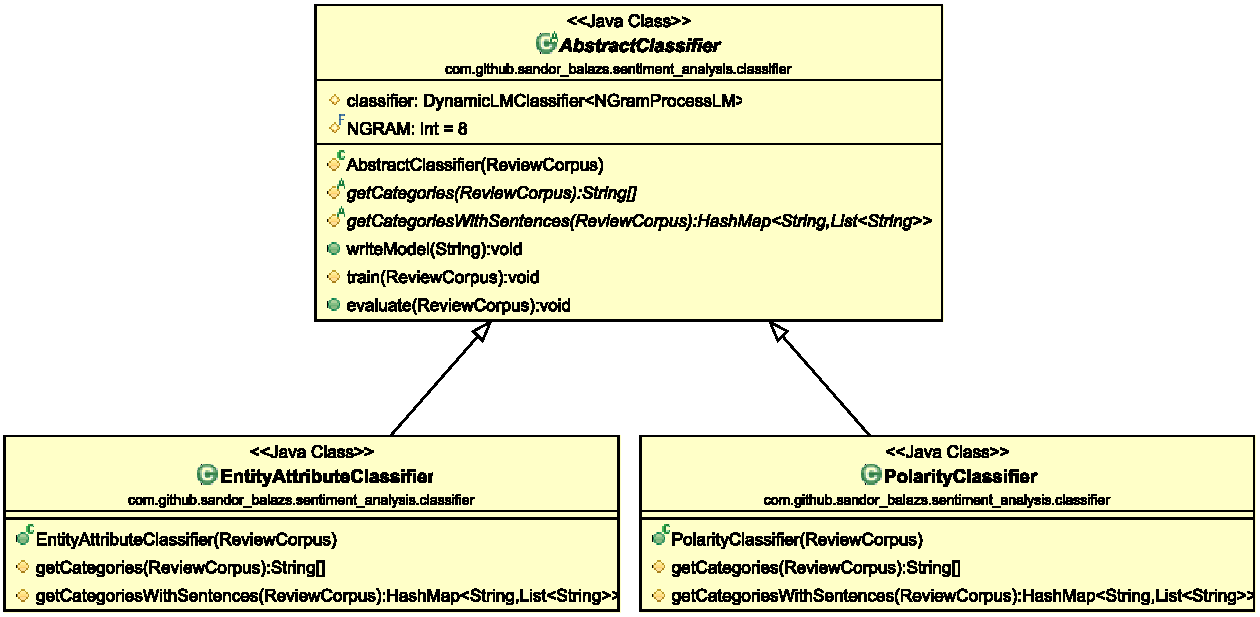
\includegraphics[width=150mm, keepaspectratio]{\resources/pdf/Classifiers}
\caption{Classifiers}
\label{fig:Classifiers}
\end{figure}

\section*{Running as an application}
Apart from testing each step separately, it is also possible to try out the
whole processing by running the Application class as can be found on Listing
\listref{application}

\begin{listing}
\begin{minted}[bgcolor=bg,xleftmargin=4pt,xrightmargin=4pt,
               fontsize=\footnotesize]{java}
# java Application Trainer.xml Evaluator.txt
\end{minted}
\caption{Running as an application}
\label{listing:application}
\end{listing}

  \bibliography{\resources/bib/site}
  \bibliographystyle{ieeetr}
  \label{page:last}
\end{document}
